\section{Emotions}

Since early 1970s, Paul Ekman and his colleagues performed extensive
studies of human facial expressions \citep{Ekman1994, Ekman1993,
Ekman1992, Ekman1992a, Ekman1979}. They studied facial expressions
in different cultures, and found several common elements in the
expression and recognition of emotions on the face of people. Specifically,
they found evidence to support universality in facial expressions
\citep{Ekman1994}. In these studies they labeled these
\textit{``universal facial expressions''} as the representation of
happiness, sadness, anger, fear, surprise, and disgust.

In 1978, Ekman and Friesen developed the Facial Action Coding System
(FACS). This is a system of coding facial expressions, done manually by
following a set of prescribed rules, where movements on the face are
described by a set of action units (AUs) \citep{Ekman1978, Ekman2002}.
The inputs are images of facial expressions, often at the climax of the
expression evoked.

{\color{Orchid}
Ekman's work inspired many researchers to analyze facial expressions by means
of image and video processing. By tracking facial features and measuring the
amount of facial movement, they attempt to categorize different facial
expressions. Recent work on facial expression analysis and recognition
(Y.Tian, T.Kanade, J.Cohn Recognizing Action Units for Facial Expression
Analysis Carnegie Mellon University, IEEE transactions on pattern
recognition and machine intelligence vol. 23, No. 2, February 2001 pp.
97-115) has used these “basic expressions” or a subset of them. In (Maja
Pantic, Leon J. M. Rothkrantz, Automatic Analysis of Facial Expressions:
The State of Art, IEEE Transactions on Pattern Recognition and Machine
Intelligence, Dec. 2000, pp. 1424 - 1444), Pantic and Rothkrantz provide an
in depth review of many of the research done in automatic facial expression
recognition in recent years. }

{\color{JungleGreen} Añadir la parte de investigaciones más recientes, quizás la
parte térmica, etc.}


\subsection{Facial datasets}

{\color{JungleGreen} Describir tipos de emociones en datasets:
emociones espontáneas/actuadas. }


\subsubsection{Cohn-Kanade AU-Coded Facial Expression Database (CK and CK+)}

{\color{Orchid} The Cohn-Kanade AU-Coded Facial Expression Database
is for research in automatic facial image analysis and synthesis and
for perceptual studies. Cohn-Kanade is available in two versions and a
third is in preparation.

Version 1, the initial release, includes 486 sequences from 97 posers.
Each sequence begins with a neutral expression and proceeds to a peak
 expression. The peak expression for each sequence in fully FACS (Ekman,
 Friesen, \& Hager, 2002; Ekman \& Friesen, 1979) coded and given an
 emotion label. The emotion label refers to what expression was requested
 rather than what may actually have been performed. For a full description
 of CK, see (Kanade, Cohn, \& Tian, 2000).For validated emotion labels,
 please use version 2, CK+, as described below.

Version 2, referred to as CK+, includes both posed and non-posed
(spontaneous) expressions and additional types of metadata. For posed
expressions, the number of sequences is increased from the initial
release by 22\% and the number of subjects by 27\%. As with the initial
release, the target expression for each sequence is fully FACS coded.
In addition validated emotion labels have been added to the metadata.
Thus, sequences may be analyzed for both action units and prototypic
emotions. The non-posed expressions are from Ambadar, Cohn, \& Reed
(2009). Additionally, CK+ provides protocols and baseline results for
facial feature tracking and action unit and emotion recognition.
Tracking results for shape and appearance are via the approach of
Matthews \& Baker (2004). For action unit and expression recognition,
a linear support vector machine (SVM) classifier with leave-one-out
subject cross-validation was used. Both sets of results are included
with the metadata. For a full description of CK+, please see P. Lucey
et al. (2010).

Version 3 is planned for future release. The original data collection
of Cohn-Kanade included synchronized frontal and 30-degree from frontal
video. Version 3 will add the synchronized 30-degree from frontal video.
}
\citep{Kanade2000, Lucey2010}


\subsubsection{Radbound Face Databases (RaFB)}

{\color{Orchid} The Radboud Faces Database (RaFD) is a set of pictures
of 67 models (including Caucasian males and females, Caucasian children,
both boys and girls, and Moroccan Dutch males) displaying 8 emotional
expressions. The RaFD in an initiative of the Behavioural Science
Institute of the Radboud University Nijmegen, which is located in
Nijmegen (the Netherlands), and can be used freely for non-commercial
scientific research by researchers who work for an officially accredited
university.

The RaFD is a high quality faces database, which contain pictures of
eight emotional expressions. Accordingly to the Facial Action Coding
System, each model was trained to show the following expressions:
anger, disgust, fear, happiness, sadness, surprise, contempt, and
neutral. Each emotion was shown with three different gaze directions
and all pictures were taken from five camera angles simultaneously.}
\citep{Langner2010}


\subsubsection{Facial Expression Recognition 2013 (FER-2013) Dataset}

In the Facial Expression Recognition Challenge (FER-2013) competitors
were invited to design the best system for recognizing which emotion
is being expressed in a photo of a human face \citep{Goodfellow2013}.
This contest introduced the Facial Expression Recognition 2013
(FER-2013) dataset. FER-2013 was created by Pierre Luc Carrier
and Aaron Courville and it is available for downlolad from official
challenge page in Kaggle
\footnote{\url{https://www.kaggle.com/c/challenges-in-representation-learning-facial-expression-recognition-challenge/data}}.

The dataset was created using the Google image search API to search for
images of faces that match a set of 184 emotion-related keywords. The data
consists of $48\times 48$ pixel grayscale images of faces, and each face
is more or less centered and occupies about the same amount of space in
each image. The task is to categorize each face based on the emotion
shown in the facial expression in to one of seven categories: anger,
disgust, fear, happiness, sadness, surprise, neutral \citep{Goodfellow2013}.

The training set consists of 28,709 examples. The public test set used
for the leaderboard of the challenge consists of 3,589 examples. The
final test set, which was used to determine the winner of the competition,
consists of another 3,589 examples.


\subsection{Face detection and feature extraction}

{\color{Orchid} Most systems detect face under controlled conditions, such as without facial
hair/glasses, any rigid head movement, the first frame should be a neutral emotion
etc, and thus nowadays, arbitrary face detection has drawn great intention
(Maja Pantic, Leon J. M. Rothkrantz, Automatic Analysis of Facial
Expressions: The State of Art, IEEE Transactions on Pattern Recognition
and Machine Intelligence, Dec. 2000, pp. 1424 - 1444).

Normally the face detection is done in 2 ways. In the holistic approach, the
face is determined as a whole unit, while in an analytic approach only some
important facial features are detected.

After the face is detected, there are 2 ways to extract the features. In the
holistic face model, a template-based method is used. In the analytic face model,
featured-based methods will be used to track the facial features while people are
showing the facial expression.}

{\color{JungleGreen} Añadir la parte de análisis más recientes, quizás con Deep
Learning o IA en general, ya directo para la detección.}


\section{Image classification considerations}

Image classification can be defined as the task of categorizing images
into one of several predefined classes, is a fundamental problem in computer
vision. It forms the basis for other computer vision tasks such as
localization, detection, and segmentation \citep{Karpathy2016}.

As this it will be seen in this section, deep learning is making major
advances in solving problems that are related on object detection and
classification in images.


\subsubsection{ImageNet Large Scale Visual Recognition Challenge (ILSVRC)}

The ILSVRC is a benchmark in object category classification and detection
on hundreds of object categories and millions of images. The challenge has
been run annually from 2010 to present \citep{Russakovsky2014}.

ILSVRC consists of two components: (1) a publically available dataset, and
(2) an annual competition and corresponding workshop. The dataset allows
for the development and comparison of categorical object recognition
algorithms, and the competition and workshop provide a way to track the
progress and discuss the lessons learned from the most successful and
innovative entries each year.

ILSVRC annotations fall into one of two categories: (1) image-level
annotation of a binary label for the presence or absence of an object
class in the image, and (2) object-level annotation of a tight bounding
box and class label around an object instance in the image. Annotating
images with corresponding object classes follows the strategy employed
by ImageNet \citep{Deng2009}.

From this annual challenge, different architectures of \textit{Deep
Convolutional Neural Networks} have been proposed and won \citep{Hinton2012,
Krizhevsky2012, Simonyan2014, Szegedy2014, Russakovsky2014}. Convolutional
neural networks will be commented on the next section, and their
architectures on the next chapter.


\subsubsection{Facial Expression Recognition Challenge (FER-2013)}

For this challenge, 56 teams submitted on the final dataset. The top
three teams all used convolutional neural networks \citep{Fukushima1982}
trained discriminatively with image transformations.
The winner, Yichuan Tang, used the primal objective of an SVM as the
loss function for training \citep{Goodfellow2013}.

Besides the competitors and winners, FER-2013 has remained as a
challenging and interesting problem, allowing people to propose
methods to solve the problem. Most of these methods use convolutional
neural network architectures \citep{Mollahosseini2015}.


\subsubsection{FaceNet Challenge}

{\color{JungleGreen} Añadir.}
\citep{Schroff2015}


\subsubsection{EmotioNet Challenge}

{\color{JungleGreen} Añadir.}
\citep{Benitez2017}


\section{Deep learning}

The previous section leads to understand what an \textit{Artificial
Neural Network} is, how it works, and how can it be use to an image
classification task.

Deep learning is a branch of machine learning. It is built on multiple
layers of artificial neural networks (ANNs) that attempt to model high
level abstractions in data \citep{Wei2017}. Deep learning methods are
representation-learning methods with multiple levels of representation:\\

\textit{``Representation learning is a set of methods that allows a machine
to be fed with raw data and to automatically discover the representations
needed for detection or classification. Deep-learning methods are
representation-learning methods with multiple levels of representation,
obtained by composing simple but non-linear modules that each transform
the representation at one level (starting with the raw input) into a
representation at a higher, slightly more abstract level''}
\citep{LeCun2015}.\\

ANNs are computational models biologically inspired by the nervous
system of living beings. ANNs can be defined as a set of processing
units (artificial neurons), linked by interconnections (artificial
synapses), that can be implemented by vectors and matrices of synaptic
weights \citep{daSilva2017}.

An ANN can be divided into three parts named layers, which are known as:

\begin{enumerate}[i]
  \item \textit{Input layer}\\
        This layer receives information (data), which can be signals,
        features, raw images, or measurements from the external environment.
        These inputs are usually normalized. This normalization results in
        better numerical precision for the mathematical operations performed
        by the network.
  \item \textit{Hidden layers}\\
        These layers are composed of neurons which are responsible for
        extracting patterns associated with the process or system being
        analyzed. These layers perform most of the internal processing
        from a network.
  \item \textit{Output layer}\\
        This layer is also composed of neurons, and thus is responsible for
        producing and presenting the final network outputs, which result
        from the processing performed by the neurons in the previous layers.
\end{enumerate}

\begin{figure}[!h]
	\centering
	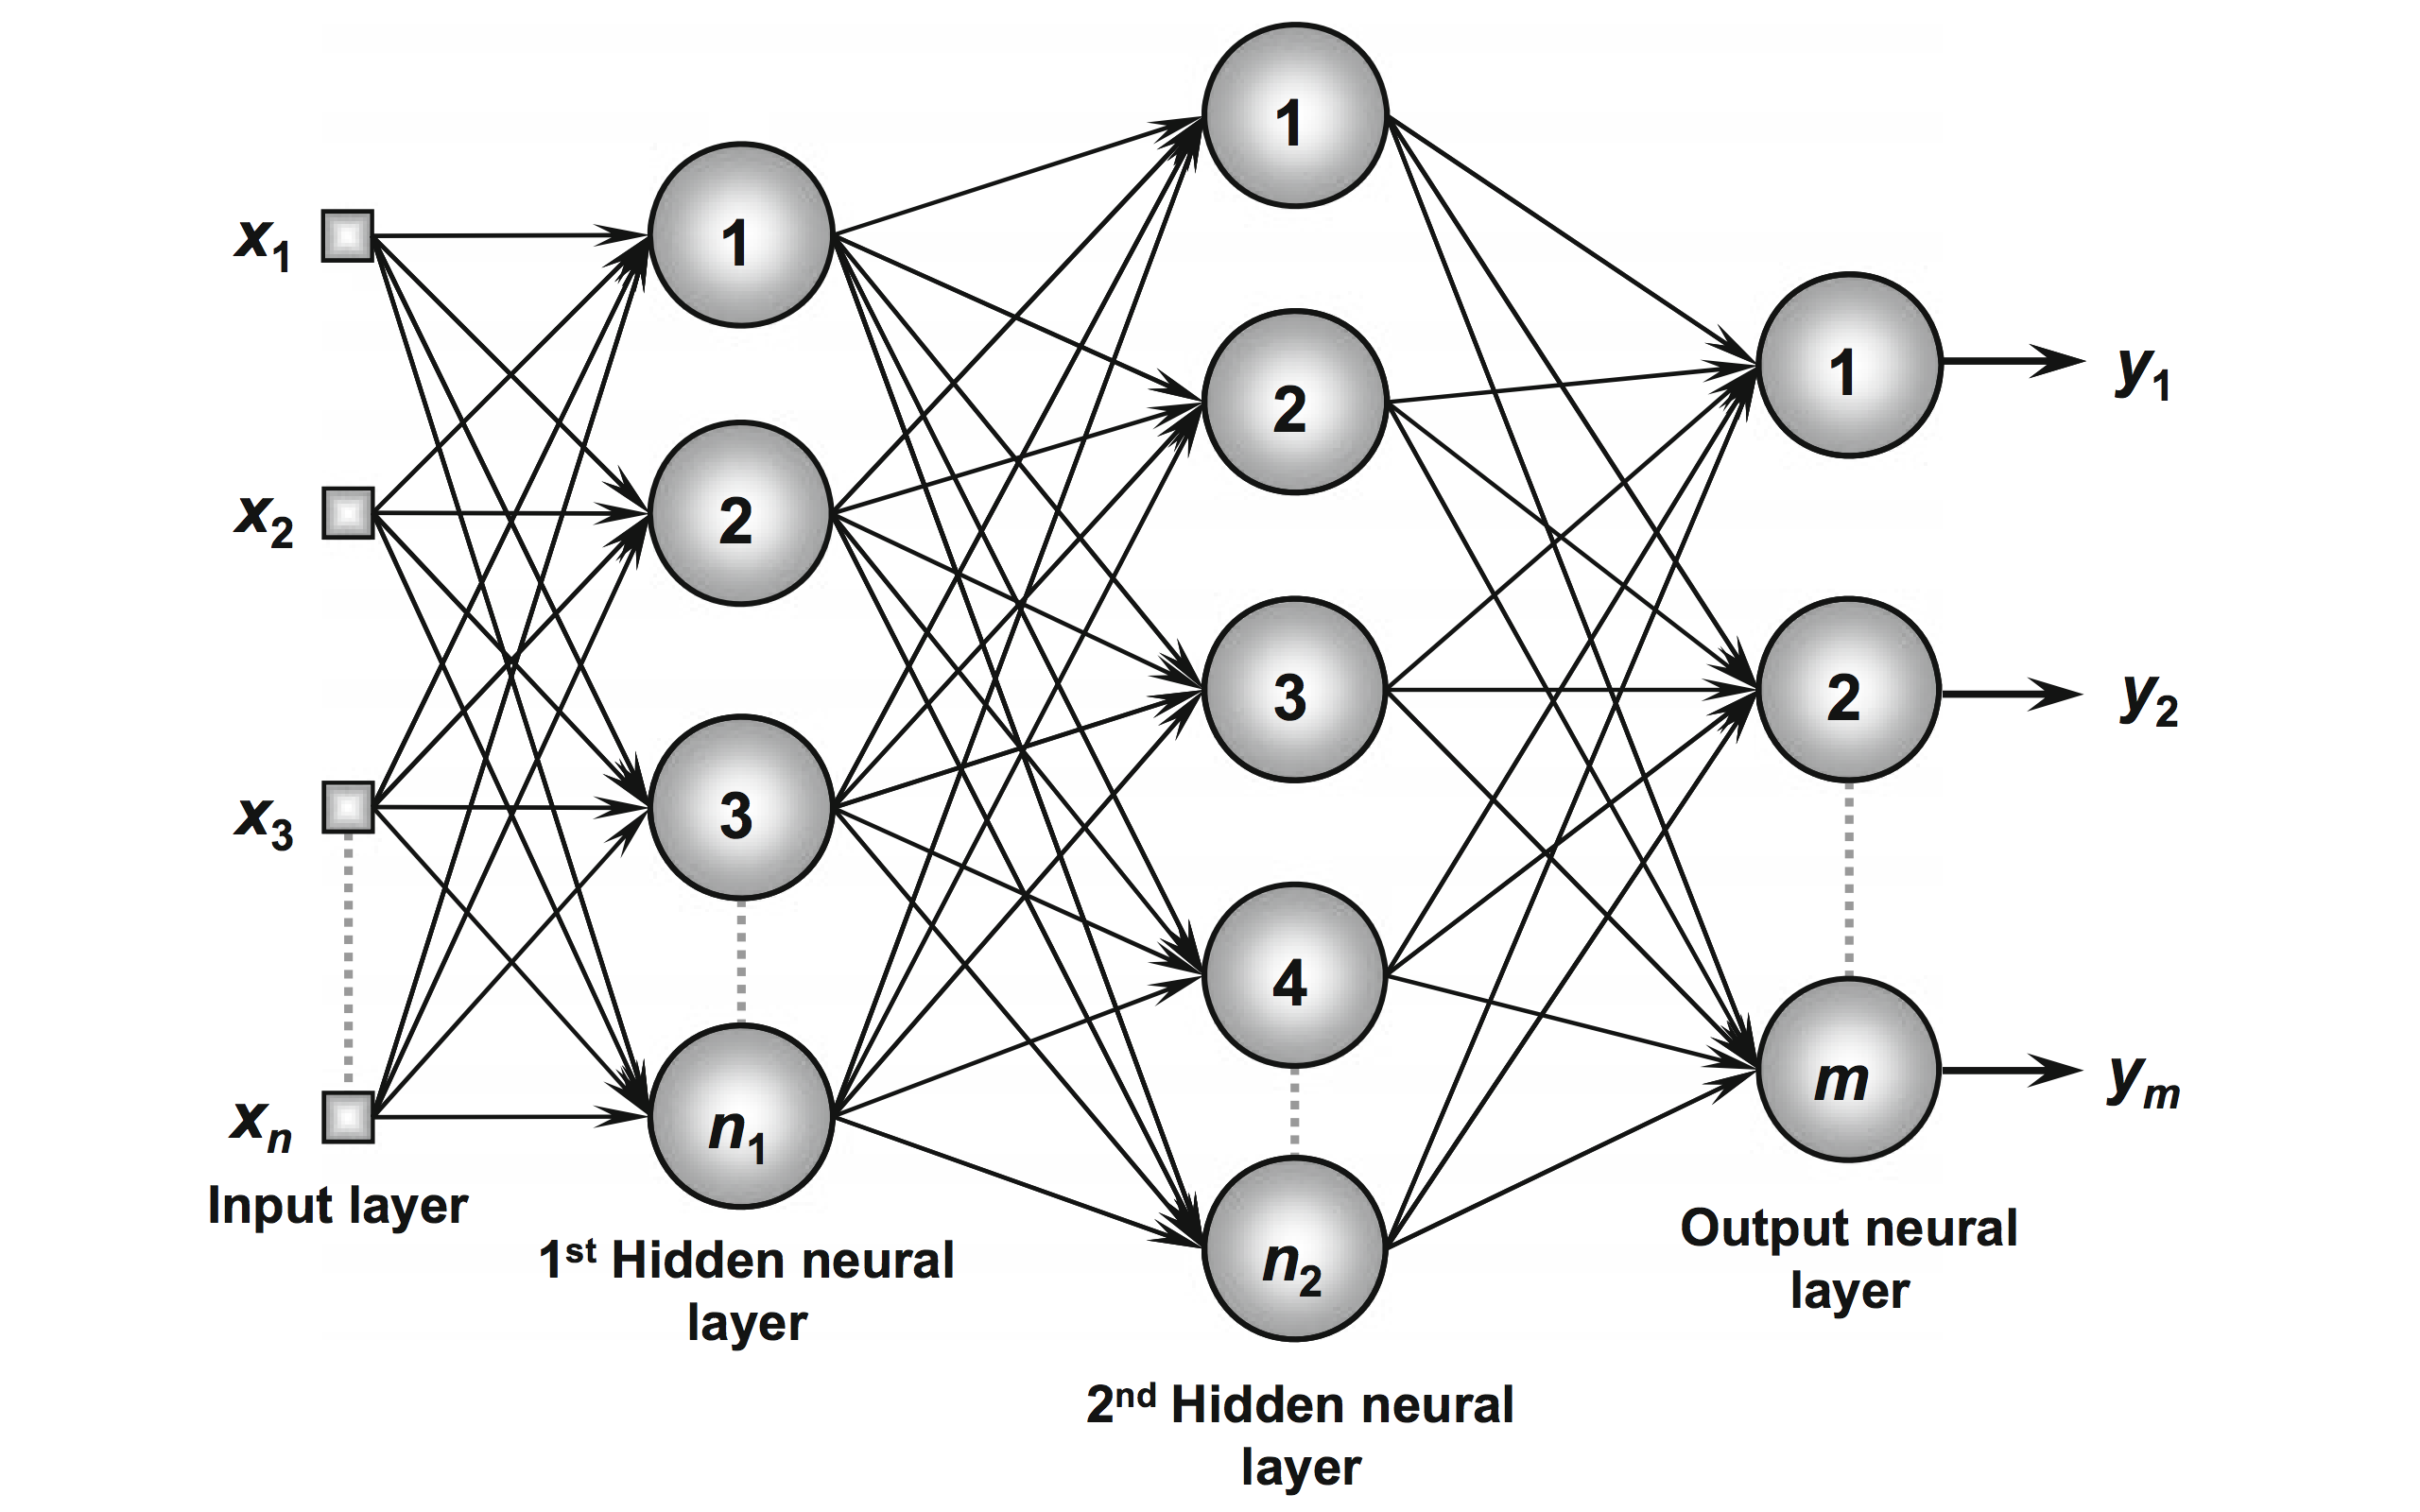
\includegraphics[width=0.90\textwidth]{ANN}
	\caption[Example of an ANN]
	{Example of a feedforward network with multiple layers
  \citep{daSilva2017}.}
  \label{fig:ANN}
\end{figure}

The architecture of an ANN defines how its several neurons are arranged.
These arrangements are structured essentially by directing the synaptic
connections of the neurons \citep{daSilva2017}. An example of an ANN in
which information flows only in one direction (a \textit{feedforward network})
can be seen in figure \ref{fig:ANN}. In this example, the flow is determined
by the direction of the arrows that connect neurons, which have associated
weights.

A deep-learning architecture is a multilayer stack of modules (\textbf{with
several hidden layers}). Most of these modules are subject to learning, which means
that the associated weights between layers can be optimized. These modules
also compute non-linear input–output mappings. Each module in the stack
transforms its input to increase the selectivity and the invariance of the
representation. With multiple layers, a deep network can implement extremely
intricate functions of its inputs that are simultaneously sensitive to minute
details and insensitive to large irrelevant variations such as the background,
pose, lighting and surrounding objects \citep{LeCun2015}.

\subsection{Convolutional neural networks}

Since the early 2000s, convolutional neural networks (CNNs) have been applied
with great success to the detection, segmentation and recognition of objects
and regions in images \citep{LeCun2015}. A relative recent practical success
of CNNs is face recognition \citep{Taigman2014}.

CNNs are feedforward networks, thus the information flows in one direction
only, from their inputs to their outputs. CNNs are biologically inspired,
as ANNs. The visual cortex in the brain, which consists of alternating
layers of simple and complex cells \citep{Hubel1959, Hubel1962}, motivates
their architecture.

CNN architectures are not unique and have several variations; however, in
general, they consist of convolutional and pooling (or subsampling) layers
grouped into modules. Either one or more layers in which neurons from the
previous layer are completely connected with each neuron of the next layer
(\textit{fully connected layers}), as in a standard feedforward neural
network, follow these modules. Modules are often stacked on top of each
other to form a deep model \citep{Waseem2017}.

An example of a simple, yet illustrative CNN architecture used for a toy
image classification task can be seen in figure \ref{fig:CNNpipeline}. This
example shows a general representation of a CNN, and describes the process
of classification on each layer.

\begin{figure}[!h]
	\centering
	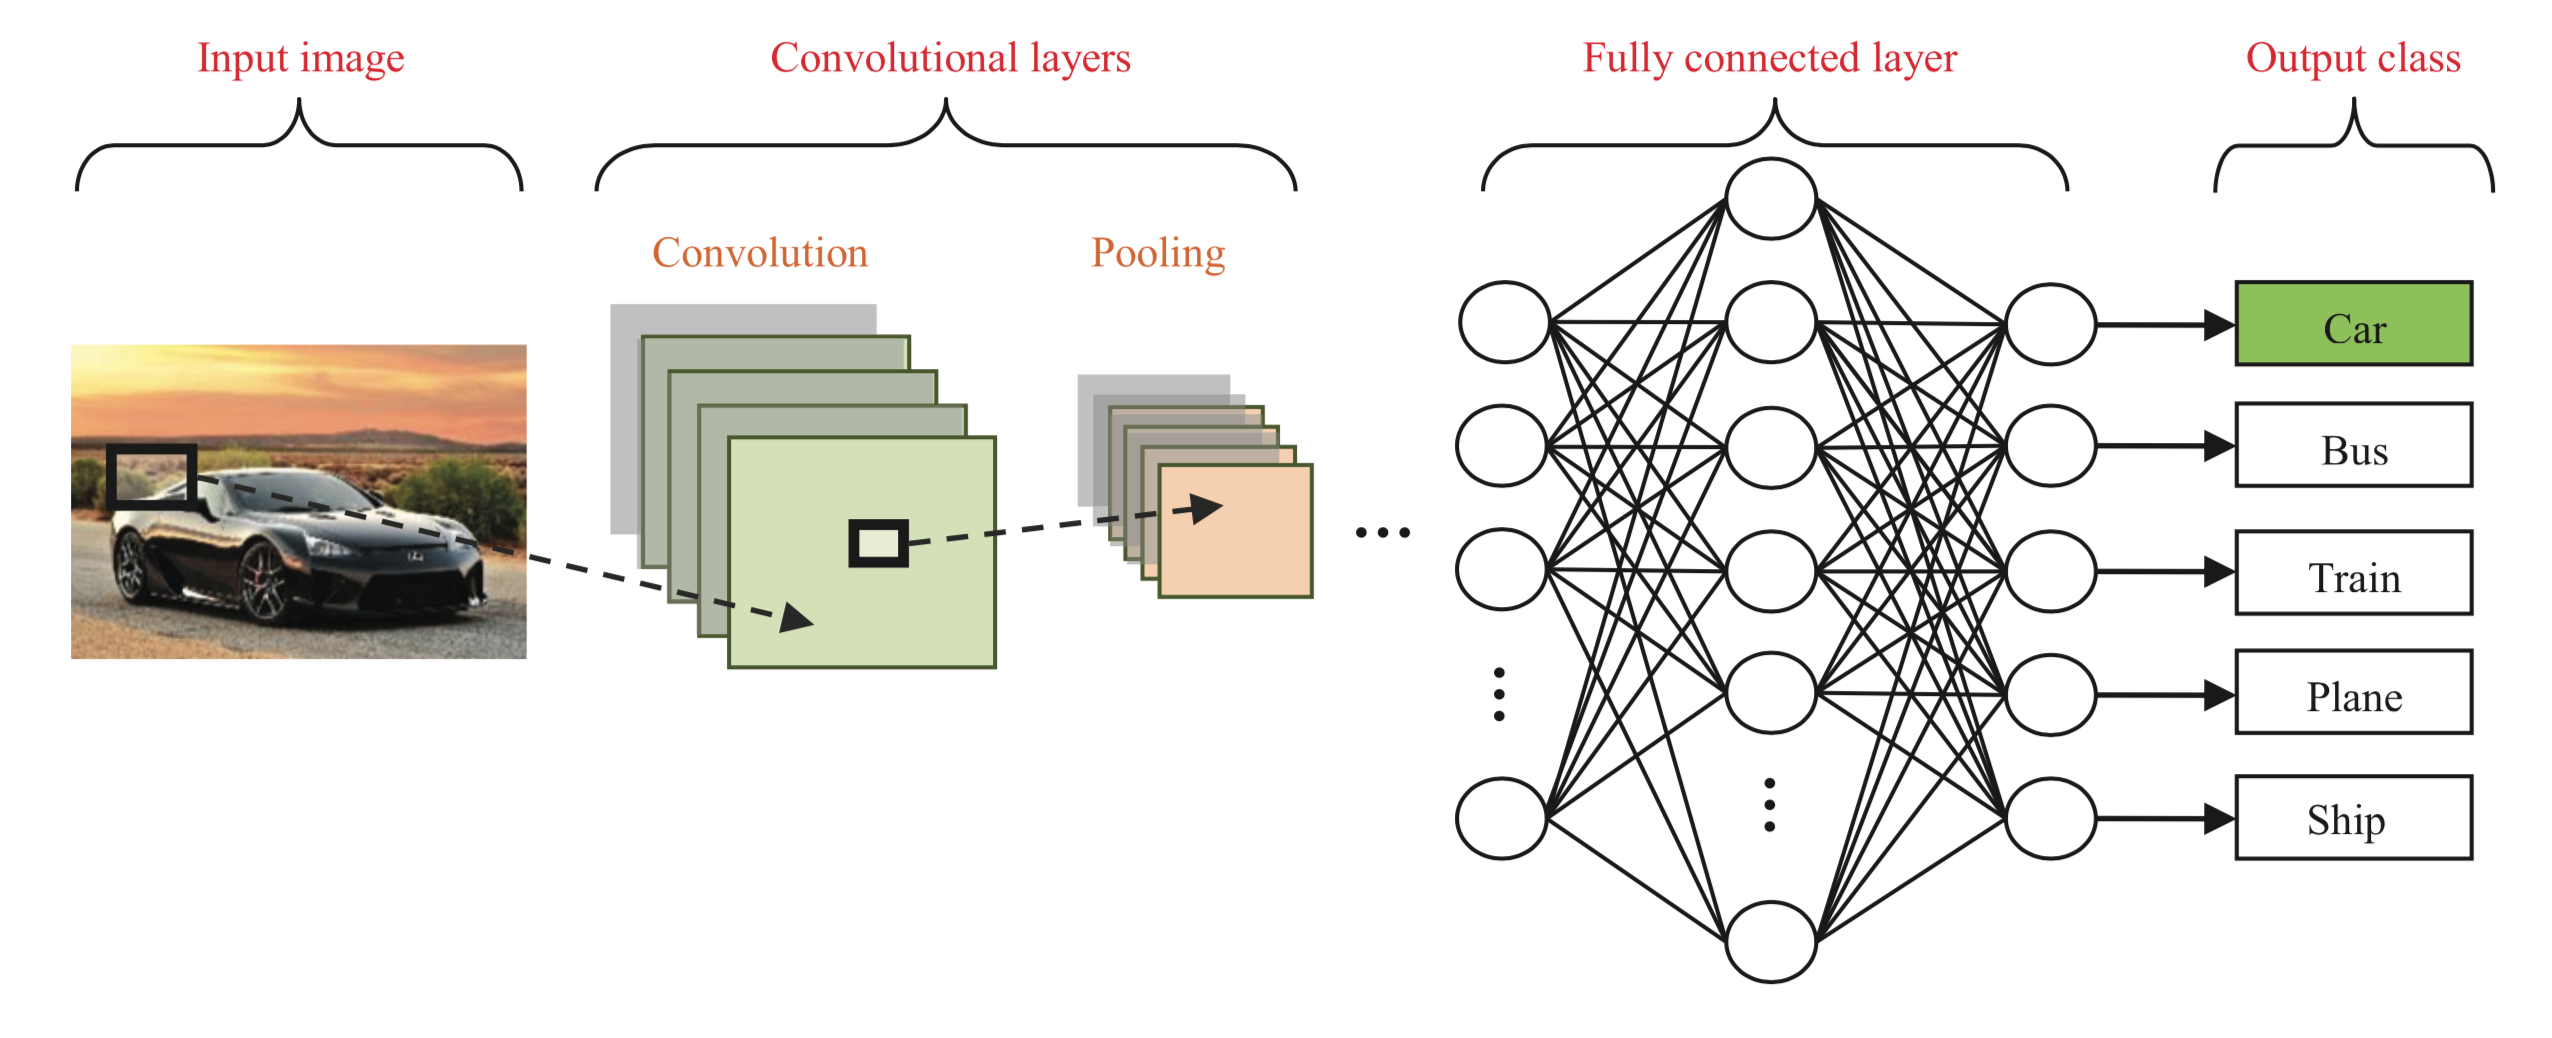
\includegraphics[width=1.0\textwidth]{CNNpipeline}
	\caption[CNN image classification pipeline]
	{CNN image classification pipeline. An image is input directly to the
  network, and this is followed by several stages of convolution and pooling.
  Thereafter, representations from these operations feed one or more fully
  connected layers. Finally, the last fully connected layer outputs the class
  label \citep{Waseem2017}.}
  \label{fig:CNNpipeline}
\end{figure}


\subsubsection{Convolutional layers}

Convolutional layers learn the feature representations of input images,
serving as feature extractors. The neurons in the convolutional layers are
arranged into feature maps. Each neuron in a feature map has a receptive
field. Each receptive field is connected to a neighborhood of neurons in the
previous layer via a set of trainable weights, sometimes referred to as a
filter bank \citep{LeCun2015}.

In order to compute a new feature map, inputs are convolved with the
learned weights. The convolved results are sent through a nonlinear
activation function $f$. All neurons within a feature map have weights
constrained to be equal; however, different feature maps within the same
convolutional layer have different weights so that several features
can be extracted at each location \citep{LeCun1998, LeCun2015}.

Formally, if the convolutional filter related to the $k$th feature map is
$w_k$, the $k$th output feature map $y_k$ can be computed as:
$$ y_k = f(w_k * x) $$

where $x$ denotes the input image. The multiplication sign in this context
refers to the convolutional operator, which is used to calculate the inner
product of the filter model at each location of the input image \citep{Yu2014}.

The extraction of nonlinear features is allowed by nonlinear activation
functions \citep{Waseem2017}. Commonly, the sigmoid and hyperbolic tangent
functions were used; but more recently, rectified linear units, or
\textit{ReLUs}, \citep{Nair2010} have become popular \citep{LeCun2015}.
Table \ref{table:actfuncs} contains some activation functions and their
respective derivatives. It must be mentioned that these and other activation
functions are commonly used since their derivatives are easy to be computed
when the learning process is done (this is introduced in the \textit{Training}
subsection).

\begin{table}[!h]
  \centering
  \renewcommand{\arraystretch}{2.4}
  \begin{tabular}{@{}lll@{}} \toprule
    \textbf{Name} \hspace{3.2cm}    & \textbf{Equation} \hspace{3cm} & \textbf{Derivative (respect to $x$)} \\ \midrule
    Identity                      & $f(x)=x$          & $f'(x)=1$           \\
    Binary step                   & $\displaystyle f(x)={\begin{cases}0&{\text{for }}x<0\\1&{\text{for }}x\geq 0\end{cases}}$ & $\displaystyle f'(x)={\begin{cases}0&{\text{for }}x\neq 0\\?&{\text{for }}x=0\end{cases}}$ \\
    Logistic (sigmoid)            & $\displaystyle f(x)=\sigma (x)={\frac {1}{1+e^{-x}}}$ & $\displaystyle f'(x)=f(x)(1-f(x))$ \\
    Tanh                          & $\displaystyle f(x)=\tanh(x)={\frac {(e^{x}-e^{-x})}{(e^{x}+e^{-x})}}$ & $\displaystyle f'(x)=1-f(x)^{2}$ \\
    ArcTan                        & $\displaystyle f(x)=\tan ^{-1}(x)$ & $\displaystyle f'(x)={\frac {1}{x^{2}+1}}$ \\
    Rectified linear unit (ReLU)  & $\displaystyle f(x)={\begin{cases}0&{\text{for }}x<0\\x&{\text{for }}x\geq 0\end{cases}}$ & $\displaystyle f'(x)={\begin{cases}0&{\text{for }}x<0\\1&{\text{for }}x\geq 0\end{cases}}$ \\
    Leaky ReLU                    & $\displaystyle f(x)={\begin{cases}0.01x&{\text{for }}x<0\\x&{\text{for }}x\geq 0\end{cases}}$ & $\displaystyle f'(x)={\begin{cases}0.01&{\text{for }}x<0\\1&{\text{for }}x\geq 0\end{cases}}$ \\ \bottomrule
  \end{tabular}
  \caption{Table with some activation functions.}
  \label{table:actfuncs}
\end{table}


\subsubsection{Pooling layers}

A pooling layer is a non-linear down-sampling, thus pooling layers reduce the
spatial resolution of the feature maps and thus achieve spatial invariance
to input distortions and translations \citep{LeCun1998, LeCun1990,
LeCun1989, LeCun2015, Ranzato2007}.

There are several non-linear functions to implement pooling, it was common
practice to use average pooling to propagate the average of all the input
values, of a small sub-region of an image to the next layer \citep{LeCun1990,
LeCun1989, LeCun1998}. Formally, average pooling computes the average
within each receptive field (in each pooling region) such that
$$y_{kij} = \displaystyle \underset{(p,q) \in \mathcal{R}_{ij}}{\text{mean}} x_{kpq}$$
where the output of the pooling operation, associated with the $k$th feature
map is denoted by $y_{kij}$, $x_{kpq}$ is the element at at location $(p,q)$
contained by the pooling region $R_{i j}$, which represents a receptive
field or sub-region around the position $(i, j)$.

In more recent models max pooling has been used \citep{Szegedy2014,
Krizhevsky2012, Simonyan2014, Zeiler2013, Xu2015}, as max pooling layers
propagate the maximum value within a receptive field to the next layer
\citep{Ranzato2007}. Formally, max pooling selects the largest element
within each receptive field (in each pooling region) such that
$$y_{kij} = \displaystyle \max_{(p,q) \in \mathcal{R}_{ij}} x_{kpq}$$
where the output of the pooling operation, associated with the $k$th feature
map is denoted by $y_{kij}$, $x_{kpq}$ is the element at at location $(p,q)$
contained by the pooling region $R_{i j}$, which represents a receptive
field or sub-region around the position $(i, j)$ \citep{Yu2014}.

Figure \ref{fig:pooling} illustrates the difference between max pooling
and average pooling. Given an input image of size $4\times 4$, if a
$2\times 2$ filter and stride of 2 is applied, max pooling outputs the
maximum value of each $2\times 2$ region, while average pooling outputs
the average rounded integer value of each subsampled region.

\begin{figure}[!h]
	\centering
	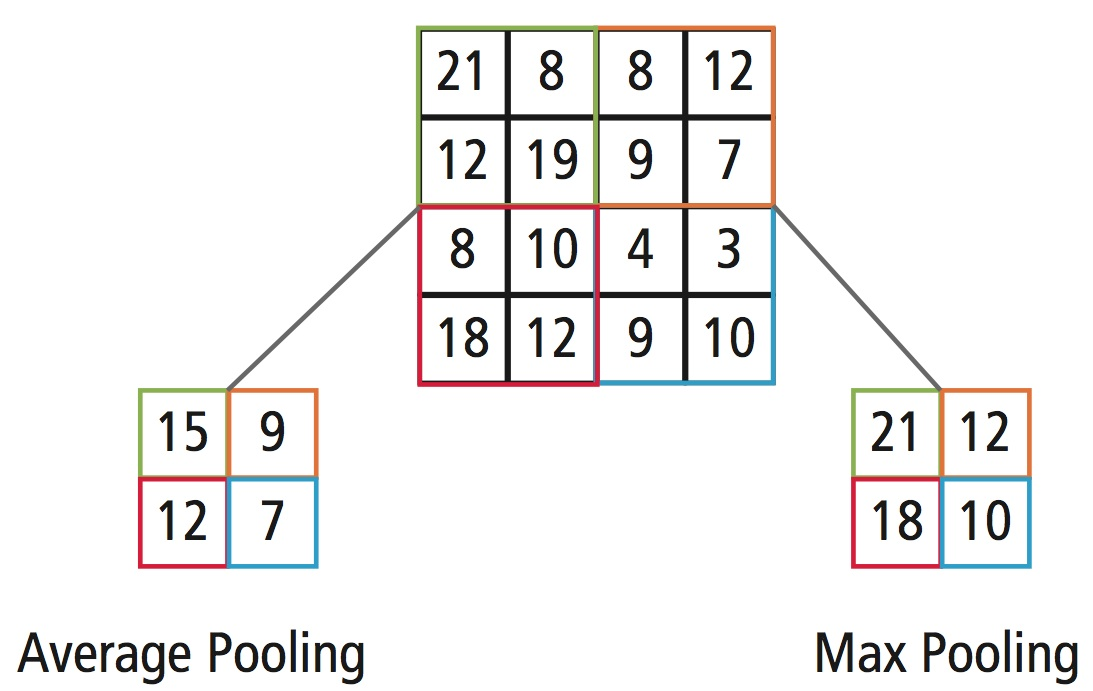
\includegraphics[width=0.70\textwidth]{pooling}
	\caption[Pictorial representation of max pooling and average pooling ]
	{Pictorial representation of max pooling and average pooling.}
  \label{fig:pooling}
\end{figure}

As new CNN models are being proposed, new pooling functions are also
proposed \citep{Lee2015, Yu2014}.


\subsubsection{Fully connected layers}

As mentioned before, convolutional and pooling layers are usually stacked on
top of each other to extract more abstract feature representations. Fully
connected layers interpret these feature representations and perform
the function of high-level reasoning \citep{Hinton2012, Simonyan2014,
Zeiler2013}.

It is quite common to use the softmax function as the activation function
for classification problems \citep{Krizhevsky2012, Lin2013, Simonyan2014,
Zeiler2013, Szegedy2014, Xu2015}. The softmax function is not function of
a single fold $x$ from the previous layer or layers. The softmax function
is defined as follows:
$$\displaystyle f_{i}({\vec {x}})={\frac {e^{x_{i}}}{\sum _{j=1}^{J}e^{x_{j}}}}
\text{, for } i = 1, \dots, J;$$
and its derivative:
$$\displaystyle {\frac {\partial f_{i}({\vec {x}})}{\partial x_{j}}}=f_{i}
({\vec {x}})(\delta _{ij}-f_{j}({\vec {x}})),$$
where $\delta$ is the Kronecker delta.


\subsubsection{Training}

In order to achieve the desired output, CNNs and ANNs use learning
algorithms to adjust their biases and weights (free parameters). The most
common algorithm used is backpropagation \citep{LeCun1998, Bengio2009,
Deng2014, DengYu2014, LeCun1989a, Srinivas2016}. Backpropagation computes
the gradient of an objective function $E$ to adjust network’s parameters
in order to minimize errors that affect performance.

The optimization of continuous non-linear functions is a widely studied
problem and there exists an extensive literature on how to solve it
efficiently, and this is why activation functions with easy-to-compute
derivatives are preferred. Most techniques involve choosing some initial
value $w_{0}$ for the weight vector and then moving through weight space
in a succession of steps of the form
$$w_{t+1} = w_t + \Delta w_t, $$
where $t$ labels the iteration step, and different algorithms involve
different choices for the weight vector update $\Delta w_t$. The simplest
approach to using gradient information is to choose the weight to
comprise a small step in the direction of the negative gradient, so
that
$$w_{t+1} = w_t − \lambda \nabla E(w_t), $$
where the parameter $\lambda >0$ is known as the learning rate, and the
value of $\nabla E(w_t)$ is evaluated at the new weight vector $w_{t+1}$
\citep{Bishop2006}.

A common problem that occurs when training CNNs is overfitting, which
is poor performance on a test set after the network is trained on
a small or even large training set. This affects the model’s ability
to generalize on unseen data. A way to avoid this is to use the dropout
method, which consists in randomly dropping units (along with their
connections) from the neural network during training \citep{Srivastava2014}.


\begin{figure}
	\centering
	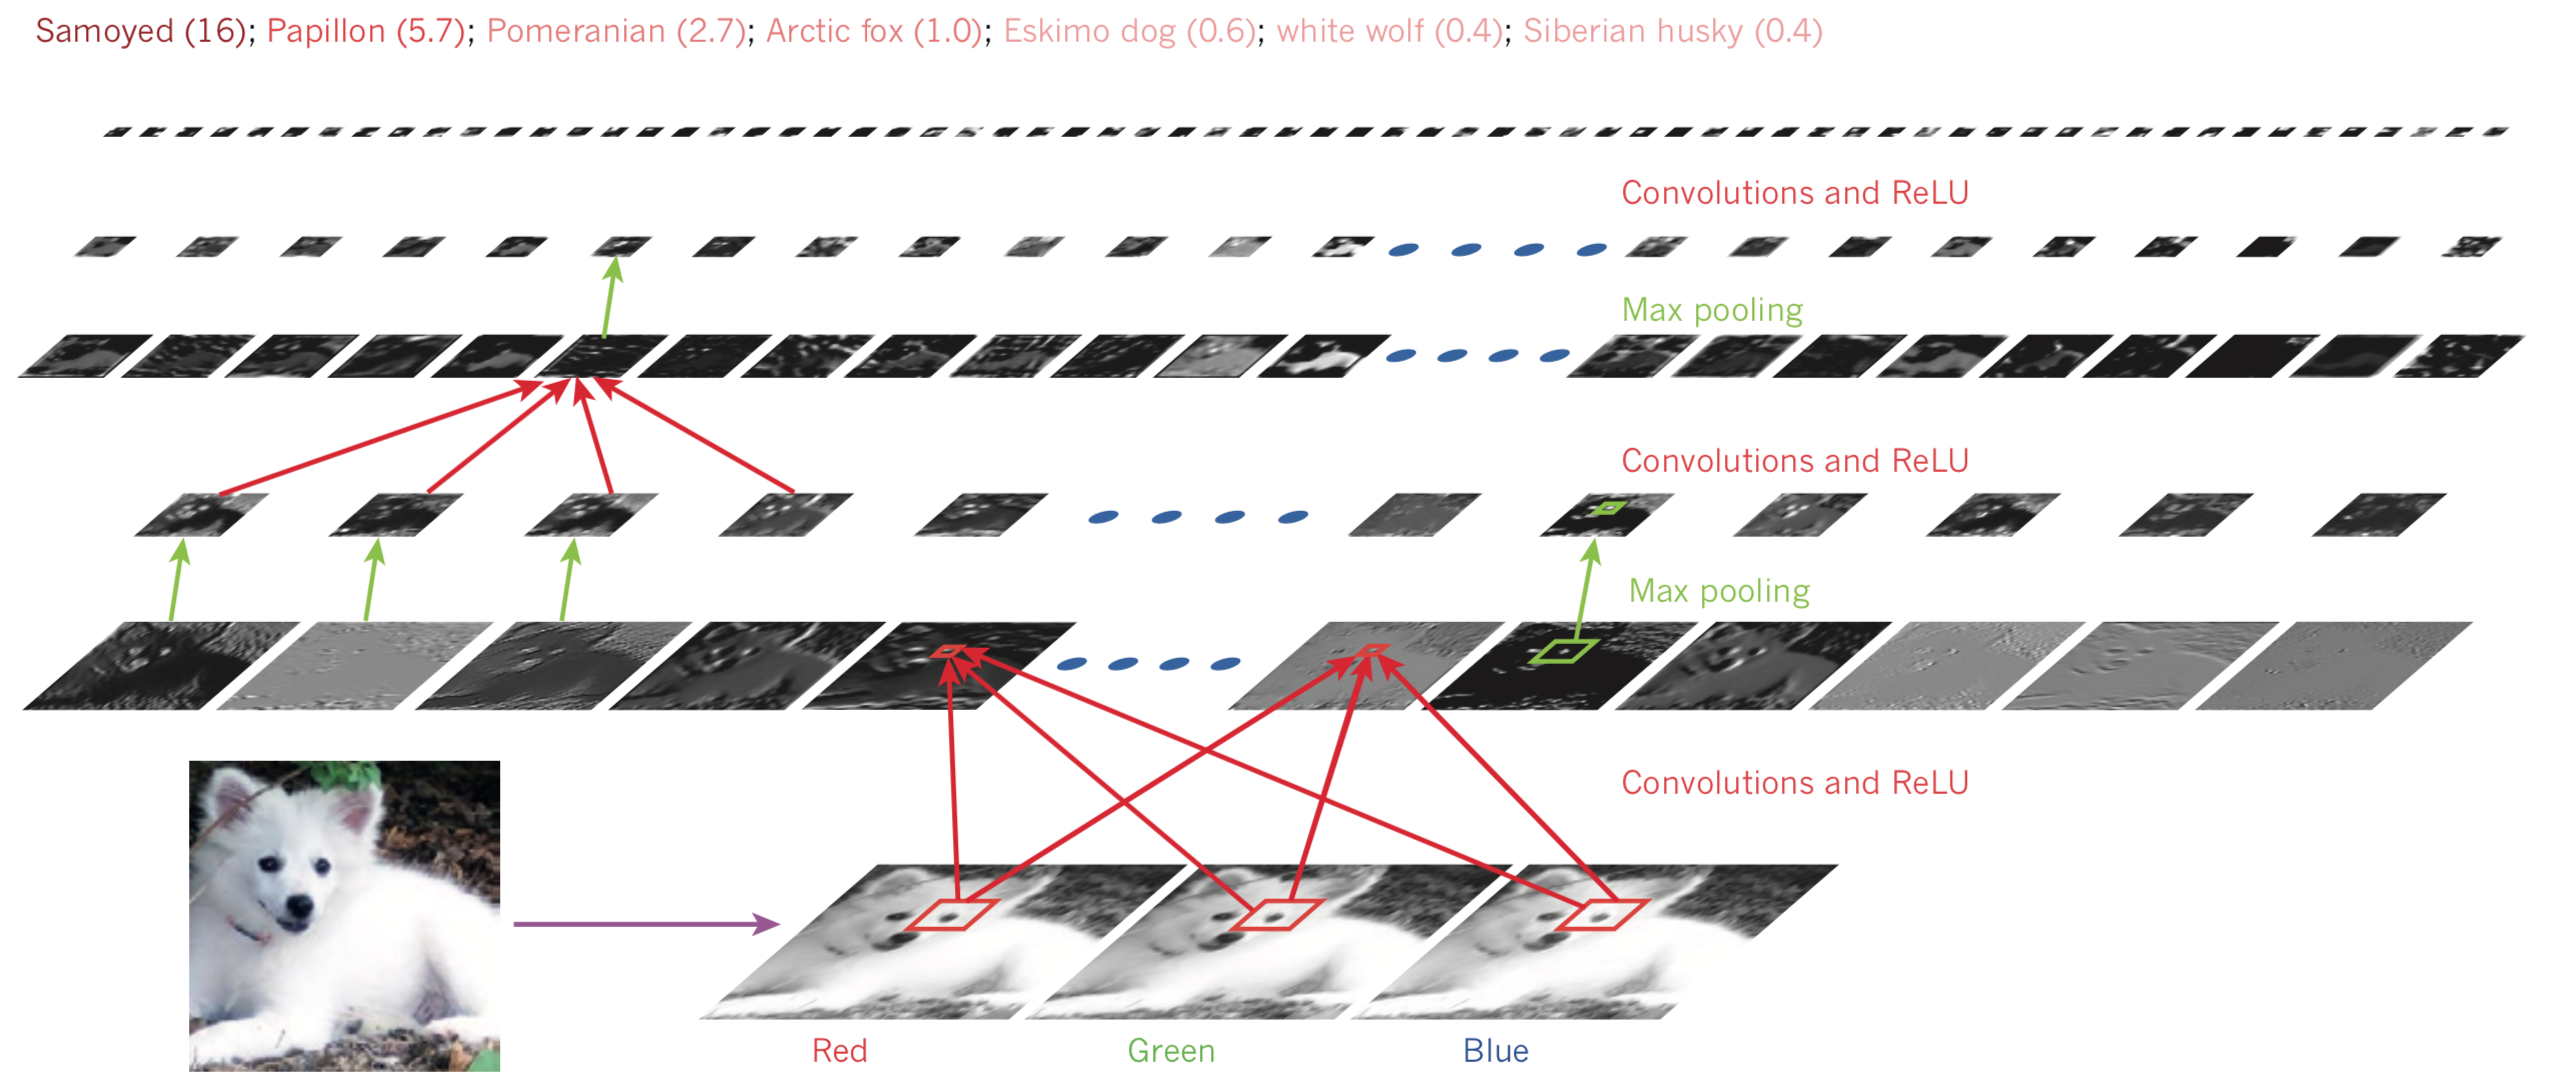
\includegraphics[width=1.0\textwidth]{InsideCNN}
	\caption[Inside a CNN]
	{\textbf{Inside a CNN.} The outputs (not the filters) of each layer
  (horizontally) of a typical convolutional network architecture applied to
  the image of a Samoyed dog (bottom left; and RGB (red, JungleGreen, blue) inputs,
  bottom right). Each rectangular image is a feature map corresponding to the
  output for one of the learned features, detected at each of the image
  positions. Information flows bottom up, with lower-level features acting
  as oriented edge detectors, and a score is computed for each image class in
  output. ReLU, rectified linear unit \citep{LeCun2015}.}
  \label{fig:InsideCNN}
\end{figure}
